\documentclass[aspectratio=169]{beamer}

\begin{document}
\begin{frame}{MTH 1020 Week 5 tutorial}
\begin{enumerate}
  \item Broad feedback on Ass 1 to start with
\end{enumerate}
\end{frame}
\begin{frame}{General feedback, assignment 1}
\begin{itemize}
  \item In future if you write your assignments by hand please \emph{scan} rather than taking a photo (there are PDF scanning apps for the phone too).\
  \item \textbf{Please submit a PDF, not a Word document.}
  \item \textcolor{red}{DO NOT USE ABBREVIATIONS AND SYMBOLS LIKE $ \implies $ AND $ \therefore $ IN THE MIDDLE OF SENTENCES.}
  \item Q1 (ii) many people missed: if you use (i), you do not need to do much more work.
  \item Q2 (a)
    \begin{itemize}
      \item simple proof: $ x + 1/x - 2 = (x - 1)^2/x $; this is positive iff $ x $ is positive. Will accept other proofs structured as a direct proof e.g. by cases,
            so long as they do not use machinery like calculus without proof.
      \item Several people used AM/GM inequality. This is not valid when one number is positive and the other number is negative, so you needed additional line to explain why the hypotheses were valid.
            In addition you should be able to prove AM/GM if required, though I will accept it here since it is not using entire new theory like calculus.
    \end{itemize}
  \item Q3 Clearly state what the inductive hypothesis is and where you use it.
\end{itemize}
\end{frame}

\begin{frame}{Assignment 1 feedback: Q1(i)}
\begin{columns}
\begin{column}{0.5\textwidth}
    \begin{center}
  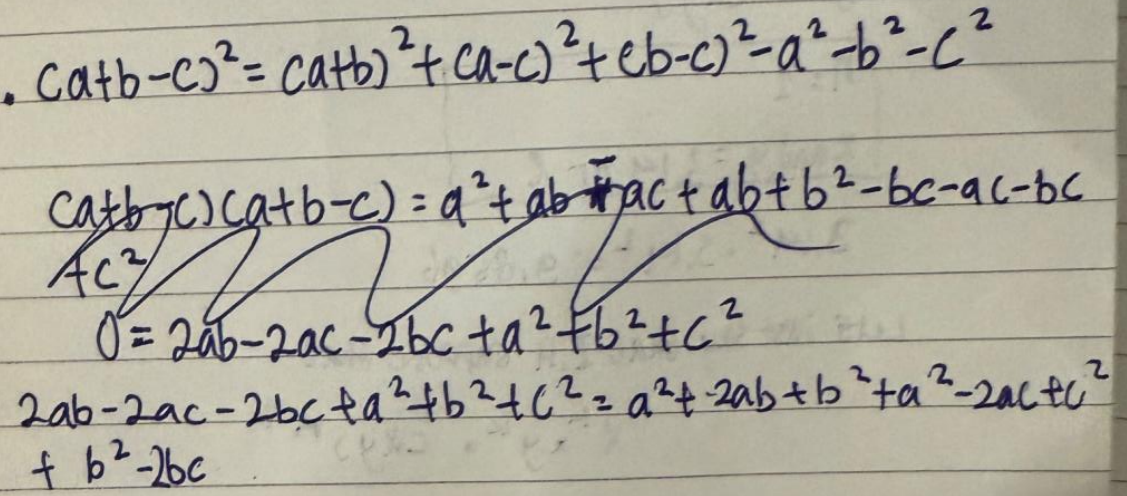
\includegraphics[width=\textwidth]{Screenshot_20250331_102924}
     \end{center}
\end{column}
\begin{column}{0.5\textwidth}
  This is not a complete proof, this is just some scratch algebra. Think about what you are trying to communicate.
%   ``Let $ a,b,c \in \mathbb{R} $. We can expand the left-hand side of the desired statement as follows:
%   \begin{displaymath}
%     (a + b - c)^2 = a^2 + 2ab + b^2 - 2bc - 2ac + c^2.
%   \end{displaymath}
%         This is equal to
%   \begin{displaymath}
%     a^2 + 2ab + b^2 - 2bc - 2ac + c^2 + (a^2 - a^2) + (b^2 - b^2) + (c^2 - c^2)
%   \end{displaymath}
%   since we are just adding $0$ three times. Observe that this rearranges to become
%   \begin{displaymath}
%     (a^2 + 2ab + b^2) + (a^2 - 2ac + c^2) + (b^2 - 2bc + c^2) - a^2 - b^2  - c^2
%   \end{displaymath}
%   and the bracketed terms factorise to become
%   \begin{displaymath}
%     (a+b)^2 + (a-c)^2 + (b-c)^2 - a^2 - b^2  - c^2
%   \end{displaymath}
%   which is the desired result.''
\end{column}
\end{columns}
\end{frame}



\begin{frame}{Assignment 1 feedback: Q1(i)}
\begin{columns}
\begin{column}{0.6\textwidth}
    \begin{center}
  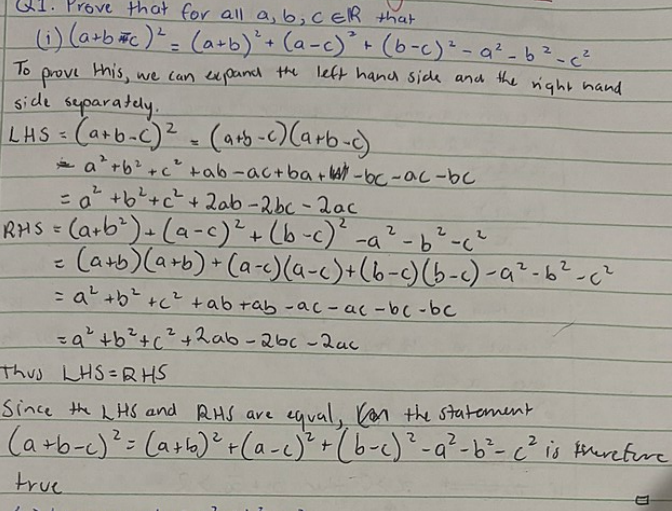
\includegraphics[width=\textwidth]{Q1a}
     \end{center}
\end{column}
\begin{column}{0.4\textwidth}
  Another attempt at Q1(i), this illustrates the kind of thing I am looking for, just a couple of sentences of explanation.
\end{column}
\end{columns}
\end{frame}

\begin{frame}{Assignment 1 feedback: Q2}
\begin{columns}
\begin{column}{0.65\textwidth}
    \begin{center}
  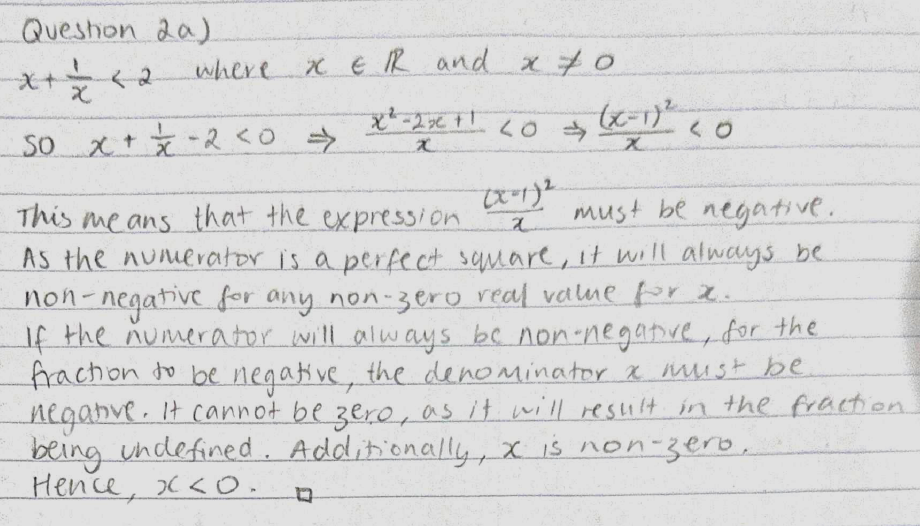
\includegraphics[width=\textwidth]{Screenshot_20250331_104130}
     \end{center}
\end{column}
\begin{column}{0.35\textwidth}
  \begin{itemize}
    \item I would add a word like ``Suppose'' at the start so it reads better.
    \item Note correct use of $ \implies $ to join logical propositions instead of to stand in for a word in the middle of a sentence.
  \end{itemize}
\end{column}
\end{columns}
\end{frame}

\begin{frame}{Assignment 1 feedback: Q3}
\begin{columns}
\begin{column}{0.5\textwidth}
    \begin{center}
  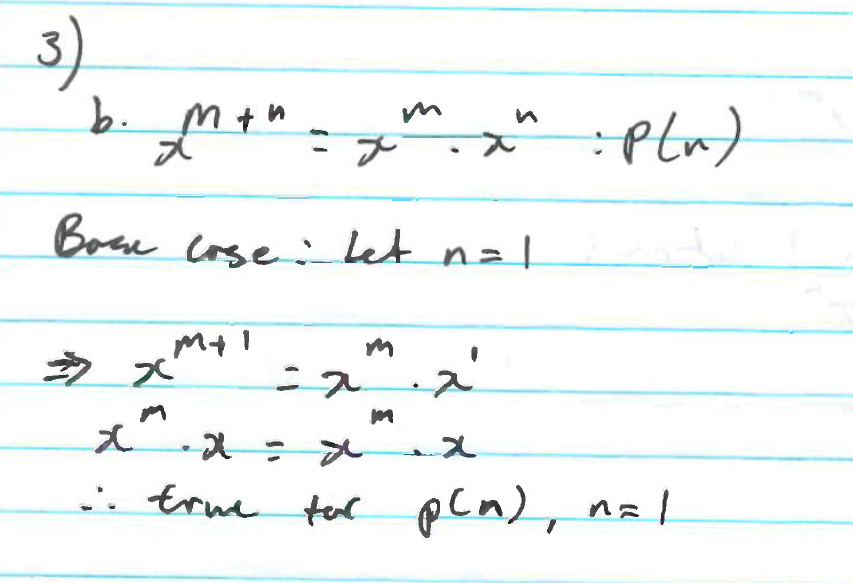
\includegraphics[width=\textwidth]{ass1q3}
     \end{center}
\end{column}
\begin{column}{0.5\textwidth}
\begin{itemize}
  \item Are you saying that $ P(n) $ is the statement ``$x^{m+n} = x^m x^n $? Say clearly what you mean. Use the examples from lectures and tutorials as a template for clear writing.
  \item What does the final line mean? What exactly is true? The reasoning is fine but remember I am looking for clear writing (audience: your average collegue in this course).
  \item (Also the case $ n = 0 $ is missed but this is a minor issue.)
\end{itemize}
\end{column}
\end{columns}
\end{frame}


\begin{frame}{Assignment 1 feedback: Q6}
\begin{columns}
\begin{column}{0.7\textwidth}
    \begin{center}
  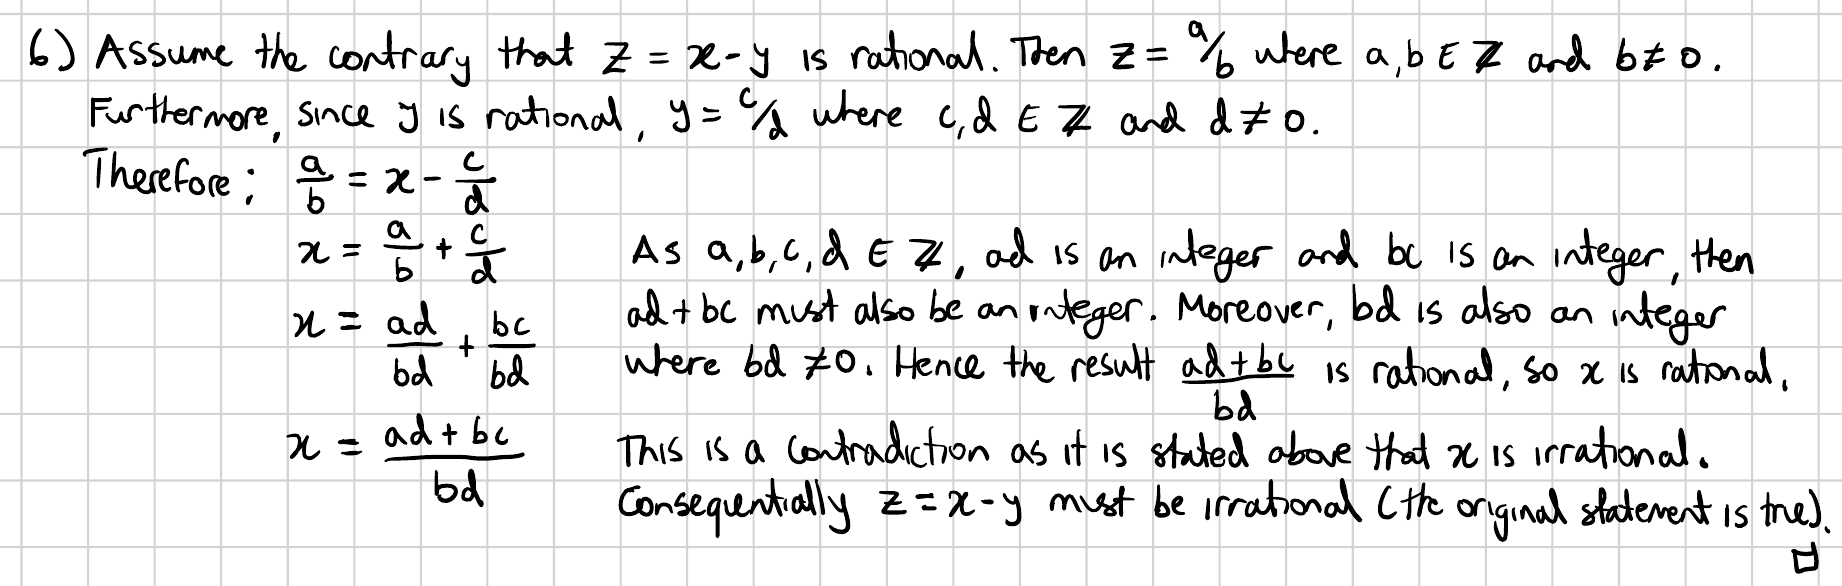
\includegraphics[width=\textwidth]{Q6}
     \end{center}
\end{column}
\begin{column}{0.3\textwidth}
  \begin{itemize}
    \item Essentially perfect!
  \end{itemize}
\end{column}
\end{columns}
\end{frame}

\begin{frame}{MTH 1020 Week 5 tutorial}
\begin{enumerate}
  \item Get into groups of 3-4 people who all prepared a different question in advance.
  \item Write your \textbf{preferred name} and \textbf{ID number} on the whiteboards so I can take attendance
  \item Present your prepared question to each other as I come around, you should only take about 5min each for this.
  \item Then get started on the other questions \textbf{in your groups}.
  \item \textbf{At the end:} please erase the boards and return any markers etc that you used (you do not need to return the handouts)
\end{enumerate}
\end{frame}



\end{document}
